%# -*- coding: utf-8-unix -*-
%%==================================================
%% chapter02.tex for SJTU Master Thesis
%%==================================================

%\bibliographystyle{sjtu2}%[此处用于每章都生产参考文献]
\chapter{情绪及情绪刺激}
\label{chap:chap2}
	


\section{情绪定义}
情绪在心理学上的定义是:人们对需求和客观事物两者关系的应激性反应,是一种每个人不同的主观感受、也是每个人都有的生理反应、还是认知的互动,并且有表达出特定的行为的趋势。同时,也有很多相关学者认为情绪和认知联系紧密,不可分割。另外,情绪表达与情绪不同,前者是一个人的内在情绪通过表情、动作、语言等方式表现出来。在意识和价值观的作用下,每个人所表达的情绪可能是强化或者弱化的真正的情绪。我们可以总结出以下几点:
\begin{itemize}
  \item 情绪是本身对外界的一种自然反应。情绪没有好坏对错,而是一种离散的对外界或者内部的刺激而自然产生的反应。
  \item 情绪是外来刺激和内在认知的一种互动。正面或负面情绪的出现,分别是自身对需求得到满足和未得到满足时产生的生理反应。这也就是情绪的生理特征。
  \item 情绪有情绪表达的趋势。情绪是由外而内的感受和刺激带来的,然后又由内而外的表达。这也就是情绪的表达和动作趋势。
\end{itemize}

\section{情绪理论}
	\centerline{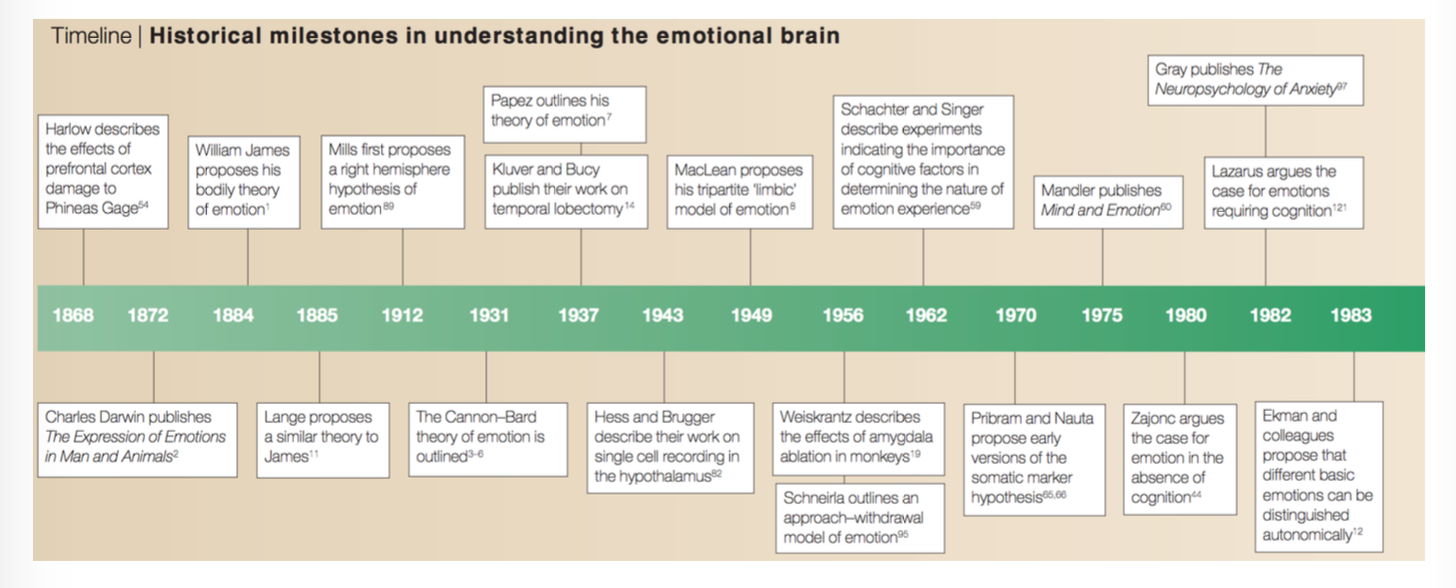
\includegraphics[width=5in]{figure/timeline.png}}
	本节将列举几个广泛使用的情绪模型:
	\begin{itemize}
		\item James Lange理论。这是发表于1884年的一篇论文,并且首次给出了情绪的定义。这个理论认为身体对外部事件产生的生理反应的结果就是情绪,是由生理学派首创的十分著名的理论。
		\item Cannon Bard理论。这个理论否定了上条理论,他们通过试验,发现无论有没有身体的响应,大脑都会产生情绪。因此,他们认为当来自外界的刺激传入到大脑之后,丘脑和大脑皮层就会被激活,从而产生了情绪。这个理论肯定了丘脑的关键作用,但是完全否定了身体和情绪的联系,这是它的不足之处。
		\item Schachter Singer理论。这个理论认为人们会对自己正在经历的情绪而产生相应的生理反应,并且注重外界环境对这种生理反应的解释。举例来说,譬如一个人在奔跑,如果是遇到了危险而逃命,那么这个理论将情绪解释为害怕;而如果是一个人跑向他喜欢的人,那么可以将这个情绪解释为激动。
		\item Opponent Process理论。不同于上述所有,这个理论从对比和对立的角度解释情绪的产生。每个人的基本情绪都有对立的情绪,当某种情绪特别突出,压过了它的对立部分,那么我们就认为自己产生了这个情绪。这个理论十分适合解释吸毒成瘾,吸毒上瘾者为了不断体验到毒品带来的感受,就会不断的吸毒,并且越来越严重。
		\item Papez Maclean理论。 Papez提出了环路理论,解释了整个情绪产生的通路,也就是从外部的刺激到产生情绪信号的大脑内部的整个通路。 Maclean在这个基础上又提出了内脏脑,它的职能是调节与情绪相关的组织和器官,并且通过丘脑调节内脏和骨骼的相应反应。
	\end{itemize}
\section{情绪分类与情绪分类模型}
	一直以来,都有两种不同的观点来进行情绪的度量。一种认为情绪是离散并且是可以相互叠加从而派生出新的情绪的。另一种是认为情绪是连续的并且可以进行测量,他们之间只有强度的差别。本论文的基本观点是情绪可以分成多个类别的。
	\centerline{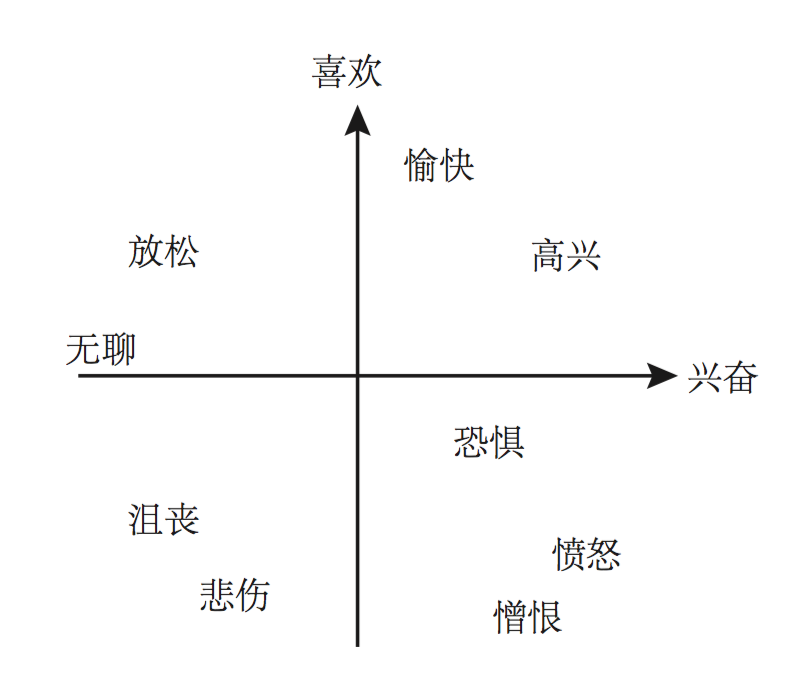
\includegraphics[width=3.5in]{figure/emotion.png}}
	 \subsection{基本情绪}
	 P. Ekman提出的理论认为情绪是离散可叠加并且可以独立的被测量。他最有影响力的研究成果是有六类基本情绪是跨越了种族和国界而广泛适用于人类中的,基于他的研究成果,他提出论点认为人的情绪需要分成六种:愤怒,悲伤,高兴,恐惧,厌恶和惊愕。 而James的情绪集合却包括了愤怒,恐惧,悲伤等\upcite{emotion}。Clynes的情绪集合包括了愤怒,厌恶,悲哀,快乐,浪漫,仇恨,中性等等。Izard的情绪集合包括了愤怒,悲伤,害怕,关心,内疚,快乐等等。
	 
	 不但情绪的划分如此众口不一,我们还很难找到明确的标尺去区别不同的情绪。随着这些年科研工作者的努力,我们才渐渐可以得知不同情绪之间的联系。譬如愤怒的情绪可以转变成为悲伤的情绪。为了让这种关联可视化,我们采用Lange的情绪分类模型,见上图。纵坐标表示的是人们的愉悦度,从厌恶到喜欢。横坐标表示兴奋程度,从低迷到兴奋。这样一来,多种不同的情绪就可以分解开来,通过这个两维度的坐标系显示出来。
	 
	 特别地,J. Panksepp在上世纪提出了大脑中情绪的定义,给出了四种最基本的情绪系统,并且认为这是四种动物出生后不久就拥有的。
	 \begin{itemize}
	 	\item 寻找。 寻找的情绪让情绪的产生者对认识世界充满了好奇,并且进行目的驱动下的寻找,从而找到生存的环境和物品,生存下去。
		\item 害怕。害怕的情绪对疼痛等外界刺激做出反应,害怕情绪的产生会造成战斗,逃遁或者颤栗的行为。
		\item 愤怒。愤怒的情绪通常由于沮丧,外部刺激,身体自由的限制等等引起。
		\item 恐慌。恐慌的情绪通常用于和母亲的分离而引起,它会造成哭泣,叫喊等等行为。
	 \end{itemize}
	 \subsection{多维度情绪表示}
	 利用数据可视化的原理,我们可以在二维模型上将所有情绪描述出来。自然地,相似的情绪状态在二维坐标系中应该距离更近,而相差愈大的情绪状态在坐标系中应该距离更远。通常,心理学家们把这两个用于可视化情绪的维度分别叫做警觉度和效价。后者主要表示情绪的消极/积极程度,而前者代表情绪给人带来刺激的强度。可以用下图(图2-1)表示。
	 \subsection{情绪}
	 虽然在每天平淡的生活中,每个人无时无刻都不被感情充斥着,但是感情却很难完全由自己控制。因此,在实验搜集数据时,我们对能够快速调动并激发实验参与者某些特定情绪和感情的方法有迫切的需求,并且要有较好的可依赖性,鲁棒性和可持续性。在观察了现有研究者尝试过的多种方法以后,论文决定采用视频库作为被试者观看的素材,也就是刺激材料。
	 通过广泛的搜索,本文作者找到了大量汉语作为音频的国内外电影或微电影,排除对英语接受程度不同这个额外变量的影响。不同于P. Ekman提出的六种基本情绪的分类,本文选取高兴,悲伤,中性三种区别最为显著的基本兴趣。在数据收集阶段,实验室通过询问大量与实验参与者各方面条件都类似的学生的评价,根据评价的高低最终选出了15段视频片段作为最终的实验素材。
	 最后,为了保证数据的可信程度和获取足够数量的数据,每个被试都分别进行三次的实验。这也为我们下一步继续研究基于个体的情绪识别研究提供了数据。
\section{本章小结}
	本章对情绪的定义,种类,分类的不同方式和情绪的二维可视化方法做了基本介绍。基于上述的情绪评价模型,本文针对相关需求使用了特定的素材,最终采集到了适合进行EEG和眼动仪信号多模态分析的数据。

